\chapter*{Ringraziamenti}

Ringrazio i miei gentili relatori, i quali -- tra una spiegazione a una correzione -- mi hanno
insegnato più cose di quante pensassi di poter imparare in una tesi triennale. Già prima di
scrivere questa tesi sapevo che il rigore matematico mi intrigava, ma avere la possibilità di
fare della \textit{fisica} rigorosa... Questo mi intriga ancora di più.

Un ringraziamento speciale va poi a mio fratello Tommaso, che dalle lontane lande umbre ha
continuato a ispirare il mio percorso di studi. Tuttavia, mi è stato riferito che la mancanza
di grafici in questa tesi gli ha suscitato grande ilarità. ``Una tesi di fisica deve contenere
dei grafici", dice. Questo è inaccettabile e mi costringe a chiedere aiuto al mio caro amico
Mattia, il quale sta esplorando temi adiacenti a quelli coperti in questa tesi. Ecco quindi
un bel grafico colorato:

\begin{figure}[h]
	\centering
	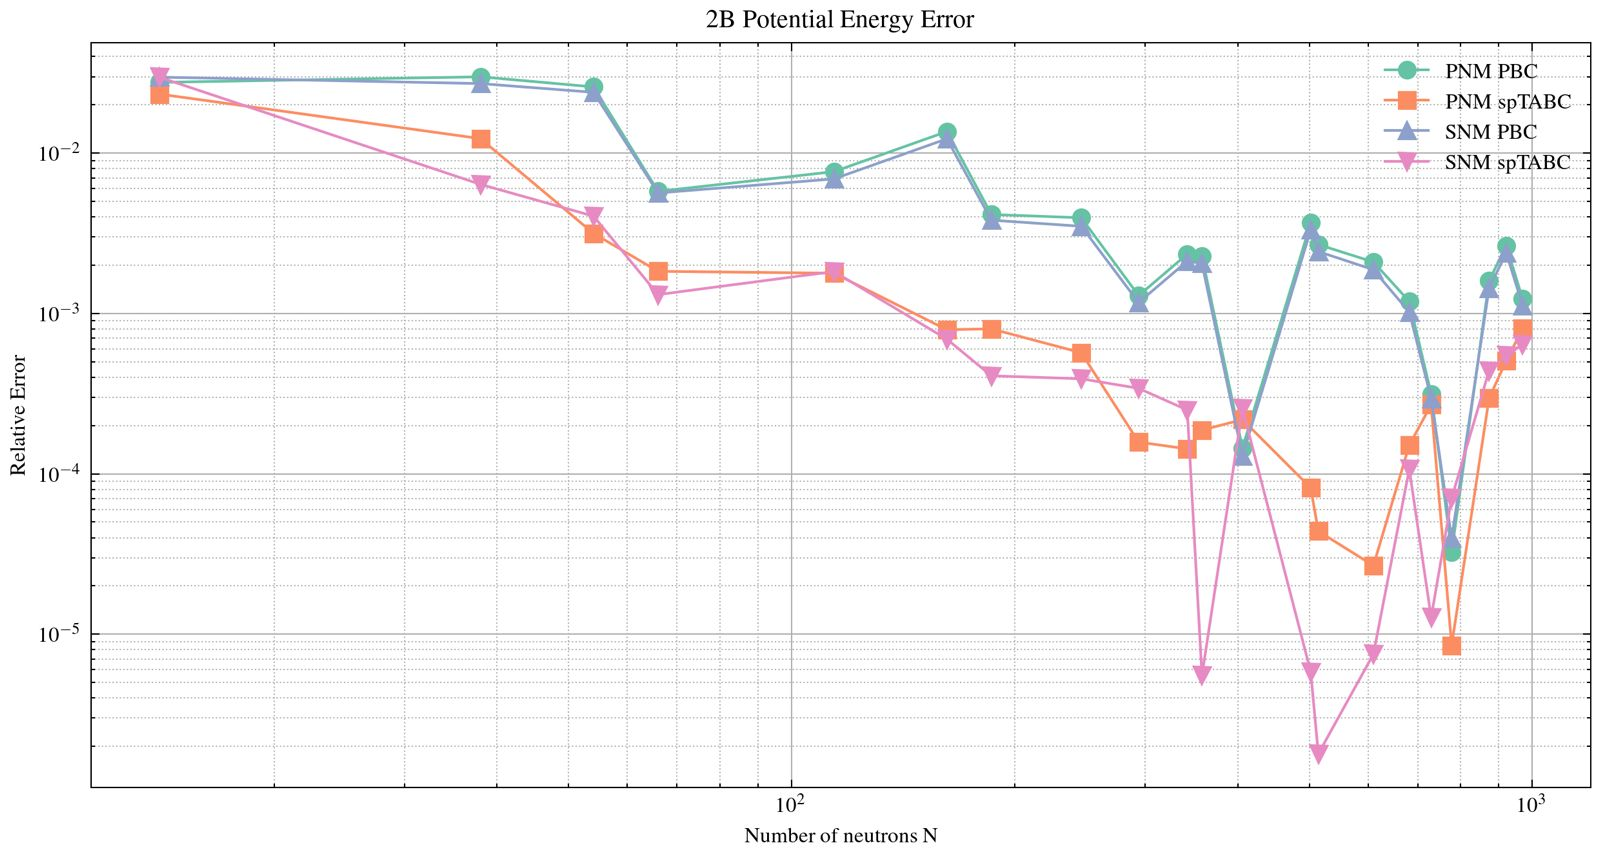
\includegraphics[width=.8\linewidth]{grafico-tia.jpeg}
	\caption{In figura è rappresentato l'errore di una simulazione del ground state di un
	sistema di molti fermioni che interagiscono tramite termini a due e a tre corpi. Le
	diverse simulazioni sono state eseguite per sistemi di materia puramente neutronica (PNM)
	e di materia simmmetrica (SNM), ciascuna approssimando il ground state di Hartree-Fock
	usando condizioni periodiche al contorno (PBC) o quasi-periodiche (Twist Angle Boundary
	Conditions). Il \textit{twist angle} viene usato per minimizzare l'errore nel passaggio
	al limite termodinamico: funge, in pratica, da regolarizzatore.}
\end{figure}
